\chapter{実験}
\label{chap:exeperiment}


\section{実験の目的}
\label{sec:purpose}

節\ref{sec:curb}で述べたような、電力ー実行時間曲線の違いによって生じる電力を増減させたときの実行時間の変動幅の違いを利用した性能向上手法は今のところ先行研究が存在しない。そのため、本実験において蓄電池を用いて理想的な電力融通を行うことができた場合にどれほどの効果があるのかを見積もることが第一の目的である。また同じく節\ref{sec:curb}で述べたように、プロセッサの周波数が離散的な値しか取ることができないことによって生じる余剰電力を利用した効果もあると予想されるため、その効果もできる限り個別に評価する。これが第二の目的である。

以下、これら二つの目的を達成するための実験方法及びその結果・考察について述べる。


\section{実験方法}
\label{sec:method}

本手法を用いた性能向上を実現するためには以下の3つの段階を踏む必要がある。

\begin{enumerate}
\item ユーザがアプリケーションのソースコードに埋め込んだフェーズ区切り文を読み取り、アプリケーションを分割する。
\item 分割されたフェーズそれぞれについて電力ー実行時間曲線を求める
\item 分割されたフェーズに対する電力融通問題を解く
\end{enumerate}

まず、1段階目について述べる。実際に節\ref{sec:phase2}のように書かれたソースコードからフェーズ区切り文を読み取るのはコンパイラレベルでの実装が必要となり困難である。そのため、本実験ではそのフェーズに入ったもしくは出た時刻をログとして出力する自作関数をソースコードに埋め込むことによって、その代わりとした。また、今回実験に利用したアプリケーションは自作のものではないので、ソースコードを読んでどの部分がフェーズの区切りであるかを完全に知ることは困難であった。そこで簡単のため、並列処理部分と逐次処理部分のみをソースコードから判別してフェーズ分割を行った。そして、プロセッサの取りうる全てのDVFSパターンについてアプリケーションを実行し、ログファイルを得た。

次に2段階目である。ここでは1段階目で得たログファイルから、それぞれのフェーズについて全てのDVFSパターンにおける平均電力と実行時間を得ることができる。それを用いてそれぞれのフェーズの電力ー実行時間曲線を計算した。ただし実際にはDVFSパターンは有限であるので、電力ー実行時間曲線は図\ref{fig:discrete_power_time}のようになった。

\begin{figure}[t]
 \begin{center}
  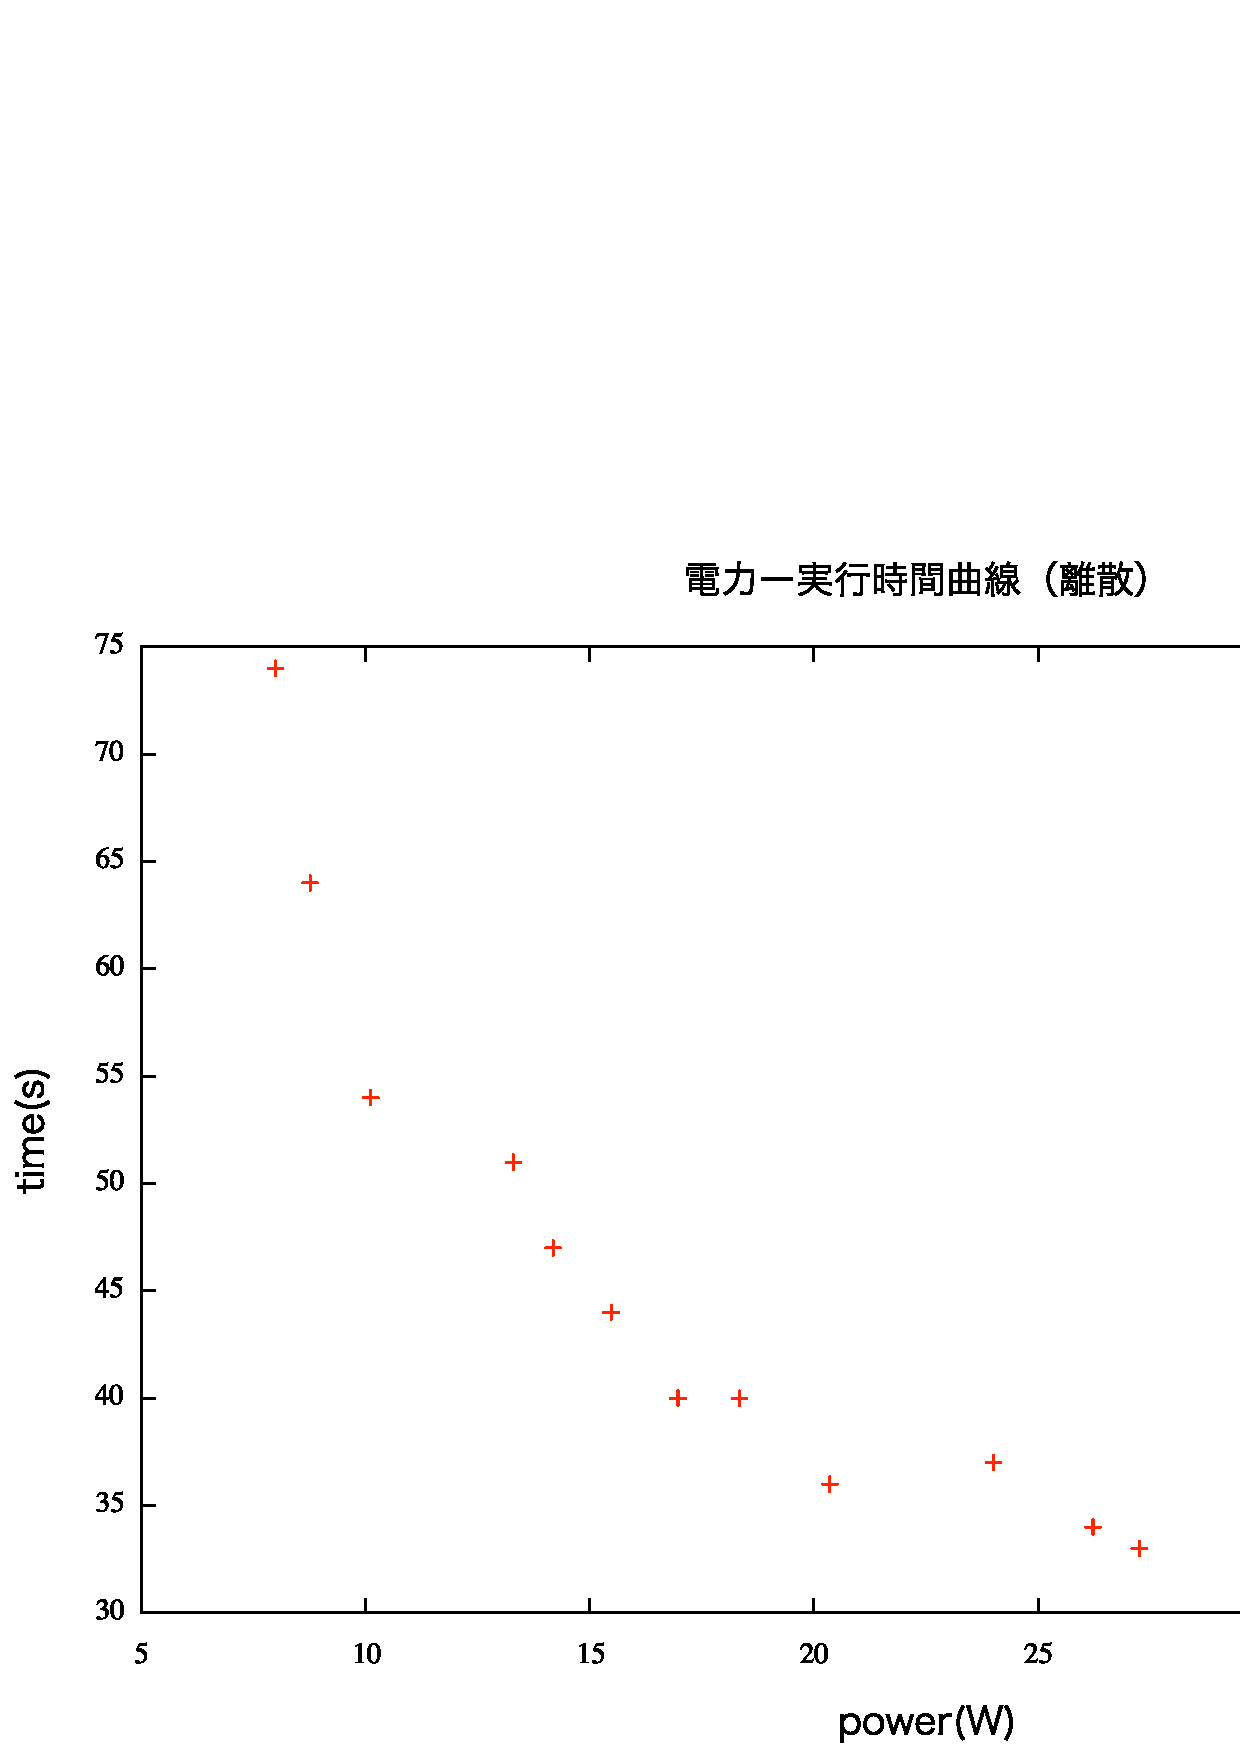
\includegraphics[width=110mm]{discrete_power_time.png}
 \end{center}
 \caption{離散的な周波数しか取れない場合の電力ー実行時間曲線}
 \label{fig:discrete_power_time}
\end{figure}

最後に3段階目は、節\ref{sec:algorithm}で述べたように得られた電力ー実行時間曲線から総当たりで最適なDVFS設定値を見つけた。

また節\ref{sec:purpose}で述べたように、本実験の目的は電力ー実行時間曲線の違いを利用した性能向上と、プロセッサの動作周波数が離散的であることを利用した性能向上のそれぞれを評価することである。ここまでの実験方法では両者の影響が入り交じった結果のみしか得られない。そこで、2段階目で得られた電力ー実行時間グラフを式\ref{asm:model}に合うように補間することによって、連続な電力ー実行時間グラフを得た(図\ref{fig:continuous_power_time})。ただし完全に連続であると電力融通問題を総当たりで解くことができなくなるため、実際にはある程度の細かい間隔で補間することで連続的な曲線への近似とした。そして、3段階目では同様に総当たりで最適なDVFSの設定値を見つけ、周波数が離散的な場合の結果と比較することによって、電力ー実行時間曲線の違いによる効果とプロセッサが離散的であることによって生じる余剰電力による効果のそれぞれを見積もった。

\begin{figure}[t]
 \begin{center}
  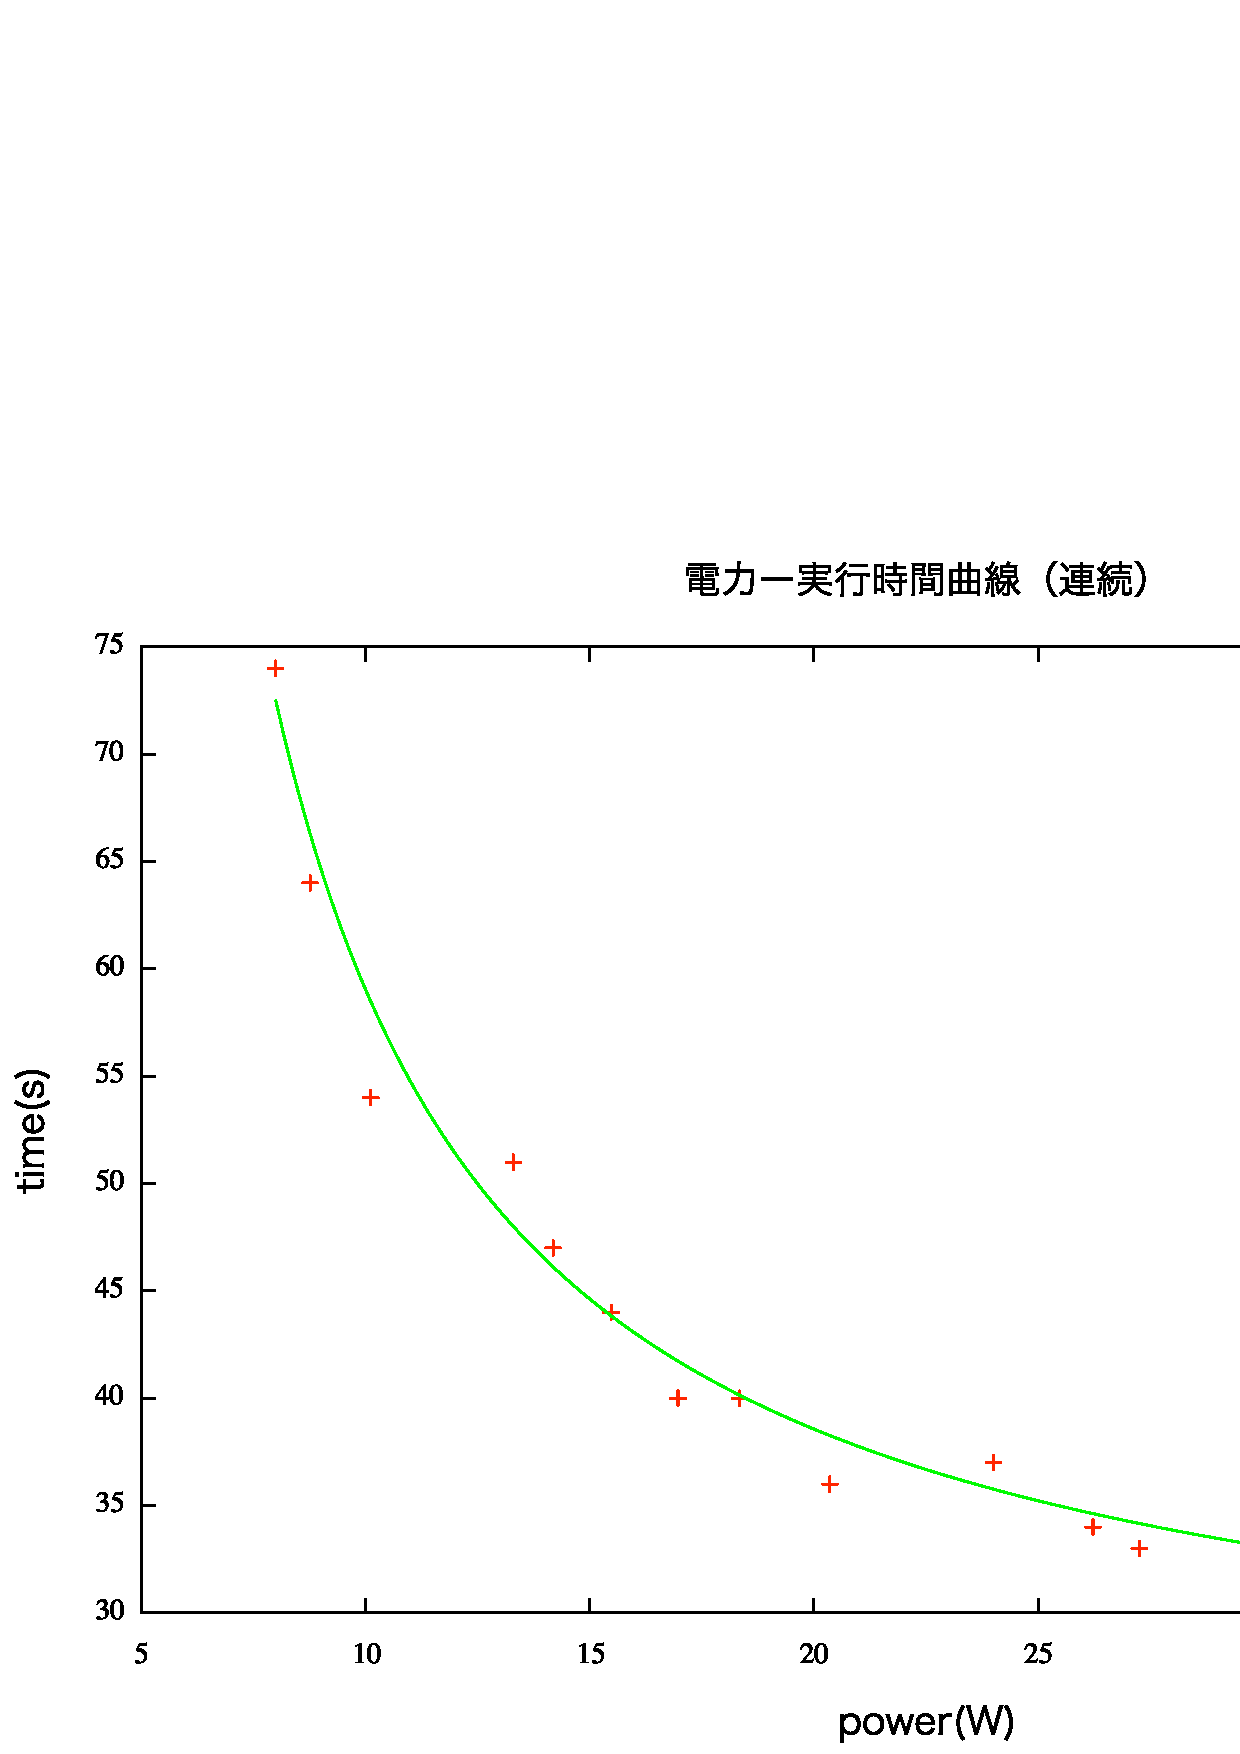
\includegraphics[width=110mm]{continuous_power_time.png}
 \end{center}
 \caption{連続補間した場合の電力ー実行時間曲線}
 \label{fig:continuous_power_time}
\end{figure}




\section{結果}
\label{sec:result}



\section{考察}
\label{sec:discussion}











